\tikzstyle{startstop}=[rectangle, rounded corners, minimum width=1.5cm, minimum height=0.5cm, text centered, draw=black, fill=red!30]
\tikzstyle{process}=[rectangle, minimum width=1.5cm, minimum height=0.5cm, text centered, draw=black, fill=orange!30]
\tikzstyle{arrow}=[thick, ->, >=stealth]

\begin{frame}{Process Steps}
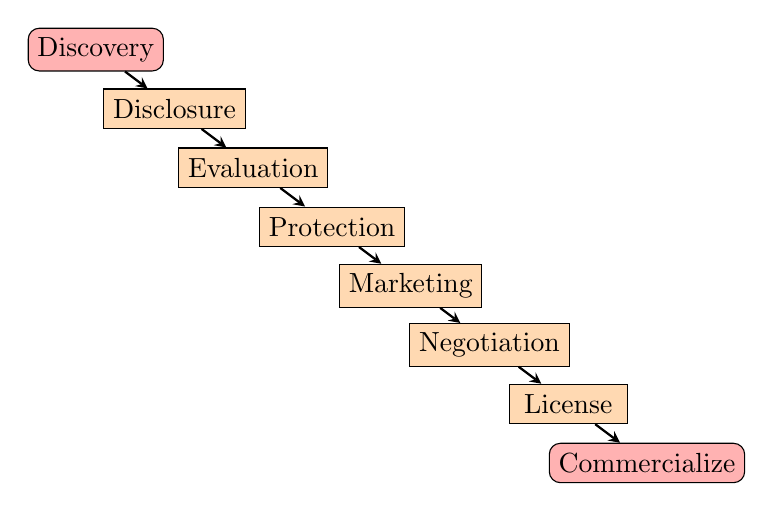
\begin{tikzpicture}[node distance=0.75cm]

\node(ps)[startstop]{Discovery};
\node(p0)[process, below of=ps, xshift=1cm]{Disclosure};
\node(p1)[process, below of=p0, xshift=1cm]{Evaluation};
\node(p2)[process, below of=p1, xshift=1cm]{Protection};
\node(p3)[process, below of=p2, xshift=1cm]{Marketing};
\node(p4)[process, below of=p3, xshift=1cm]{Negotiation};
\node(p5)[process, below of=p4, xshift=1cm]{License};
\node(pe)[startstop, below of=p5, xshift=1cm]{Commercialize};

\draw[arrow](ps)--(p0);
\draw[arrow](p0)--(p1);
\draw[arrow](p1)--(p2);
\draw[arrow](p2)--(p3);
\draw[arrow](p3)--(p4);
\draw[arrow](p4)--(p5);
\draw[arrow](p5)--(pe);

\end{tikzpicture}
\end{frame}
